% header

\documentclass[10pt,a4paper]{article}
\usepackage{amsmath,mathrsfs,mathtext} 
\usepackage[latin1]{inputenc}
\usepackage{hyperref}
\usepackage{amssymb}
\usepackage{ngerman}
\usepackage{graphicx, epsfig} 
% the document
\begin{document}

% create the title
% Please replace the data in brackets [] with actual data.
\title{Abgabe - �bungsblatt [$3$]\\
\small{Einf�hrung in die Computergraphik und Visualisierung}}
\author{ [Svetlana Shishkovets] \and [Victor Lopatin] \and [Lihn Chi Tran]}
\date{\today}
\maketitle

\section*{First Exercise}
\begin{itemize}
\item (a) $p_1,p_2 \in P(\mathbb {R}^3)$\\
Remember that $(a,b,c,d)^T= (\frac{a}{d},\frac{b}{d},\frac{c}{d})^T$ if $d\neq 0, \Rightarrow$\\
$p_1=(\frac{14}{2},\frac{3}{2},\frac{4}{2}) =(7,1.5,2) $,\\
$p_2=(\frac{12}{3},\frac{0}{3},\frac{3}{3}) =(6,0,1) $ 
\item (b) Since we cannot divide by 0(otherwise we will get vector of infinite length), we cannot represent in $\mathbb {R}^3 (a,b,c,0)$ 
\end{itemize}
\section*{Second Exercise}
We will use ideas, similar to the lecture. \\
\begin{figure}[h]
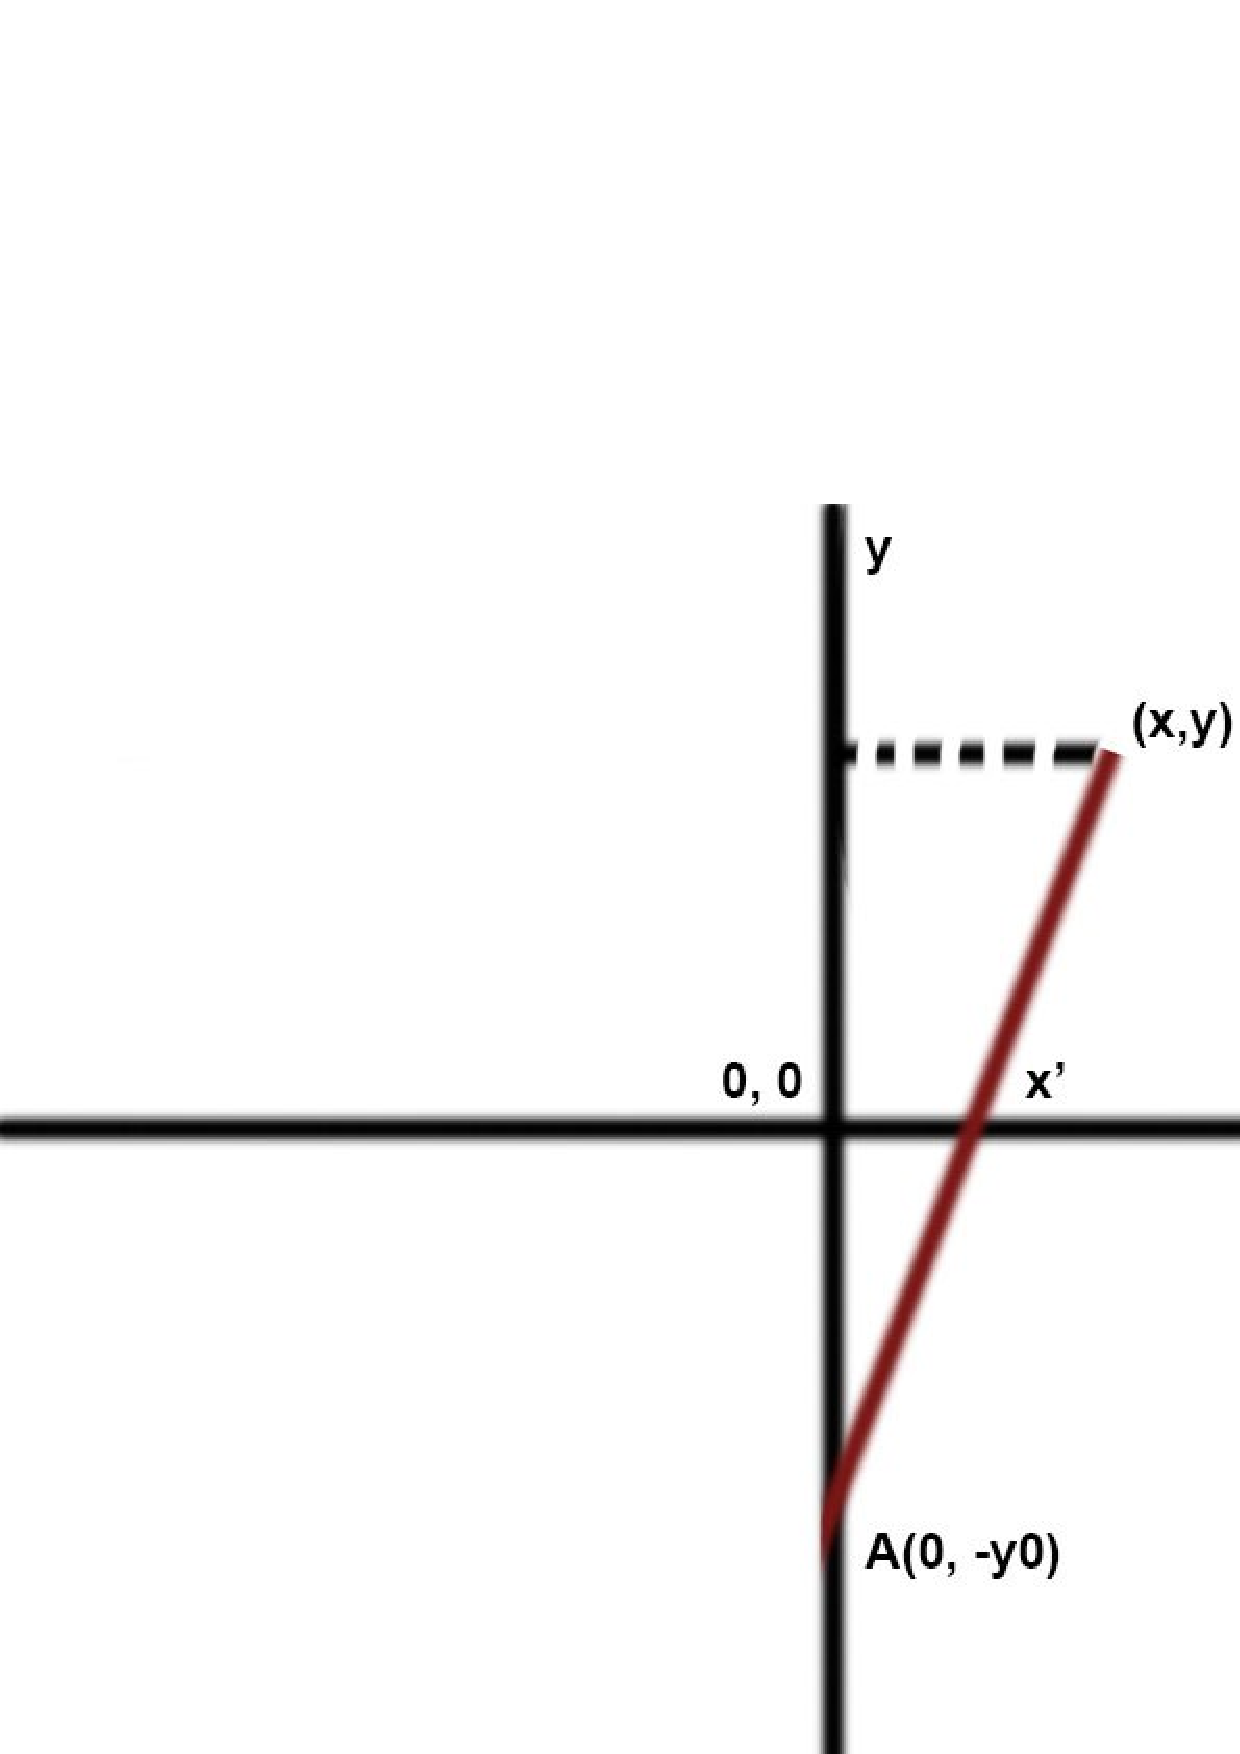
\includegraphics[scale=0.3]{1}
\end{figure}\\
$\vartriangle(A;(0; y);(x; y))\sim \vartriangle(A;(0;0);(0; x'))\Rightarrow$\\
$\frac{x'}{x}=\frac{y_0}{y+y_0} \Leftrightarrow x'=\frac{y_0x}{y+y_0}$  
\section*{Third Exercise}
Quternions $q$ and $-q$ represent the same rotation, and it can be show by reproducing the calculation of the rotation axis and angle. \\
For $-q$ the rotation of point $p$ will be written as $p'=q^{-1}pq$. \\
Thus the rotation axis has to be transformed into itself: \\
$(\cos{\theta} - r \sin{\theta}) r (\cos{\theta} + r \sin{\theta} = \cos{\theta}^2r - \sin{\theta}^2r^3 = r $ \\
And the angle is calculated as: \\
$\langle R(q), q \rangle = \langle (\cos{\theta} - r\sin{\theta}) q (\cos{\theta} + r\sin{\theta}), q \rangle = \\ = \langle\cos{\theta}^2q + \sin{\theta}\cos{\theta}r\times q \sin{\theta}\cos{\theta}q\times r - \sin{\theta}^2q , q\rangle = \\ = \cos{\theta}^2 - \sin{\theta}^2 = \cos{2\theta}$ \\
Therefore, as the axis and the angle are the same, this inverse quaternion represents the same rotation.
\end{document}
